\documentclass{standalone}
\usepackage{tikz}
\usetikzlibrary{matrix,decorations.pathreplacing, calc, positioning,fit}
\begin{document}
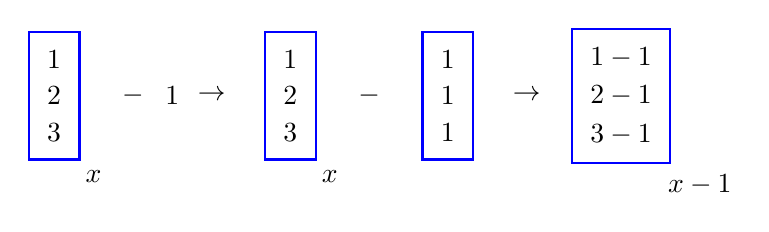
\begin{tikzpicture}[>=stealth,thick,baseline,mtxstyle/.style={matrix of math nodes, draw=blue}]
% \tikzstyle{mxborder} = [matrix of mathnodes, draw, blue];
    \matrix (A) [mtxstyle] {
    1\\
    2\\
    3\\
   };
   \node (Ax) [right=0.5cm of A.south, anchor=north] {$x$};
   \node (B) [right of = A] {$-$};
   \node (C) [right of = B, node distance=0.5cm] {$1$};
   \node (D) [right of = C, node distance=0.5cm] {$\rightarrow$};
    \matrix (E) [mtxstyle, right of=D] {
    1\\
    2\\
    3\\
   };
  \node (Ex) [right=0.5cm of E.south, anchor=north] {$x$};
   \node (F) [right of = E] {$-$};
    \matrix (G) [mtxstyle, right of=F] {
    1\\
    1\\
    1\\
   };
   \node (H) [right of = G] {$\rightarrow$};
    \matrix (I) [mtxstyle, right of=H, xshift=2mm] {
    1 - 1\\
    2 - 1\\
    3 - 1\\
   };
  \node (Ix) [right=1cm of I.south, anchor=north] {$x - 1$};

\end{tikzpicture}
\end{document}